% =====================================================================
% Chapter 5 --- EKF-Based Target Tracking in Global and Local Frames
%                                                            [tracker -- HERE]
% Narrative: derive both formulations, PROVE their equivalence under the
% stated assumptions, verify it numerically, and characterise the regimes
% where they genuinely diverge. Builds on the framework of Chapter 2.
% =====================================================================

This chapter develops the tracking stage of the pipeline introduced in
Chapter~\ref{cha:pipeline} as a self-contained estimation problem: recovering the
three-dimensional position, velocity and size of a moving object from
range--bearing measurements produced by a sensor rigidly attached to a moving
aerial platform. Two formulations of the Extended Kalman Filter (EKF) are
derived --- one that carries the object state in a global inertial frame and
one that carries it in the platform's local frame --- and their relationship is
analysed rigorously. The central result is that, under the modelling
assumptions adopted here, the two formulations are \emph{mathematically
equivalent}; we then identify the precise conditions under which a genuine
difference between them emerges. This material extends the formulation first
reported in \cite{delima2025fusion}.

\section{Tracking on a Moving Platform: The Reference-Frame Dilemma}

Consider an aerial platform carrying a sensor (a depth or stereo camera, or a
camera fused with a LiDAR) that, at each discrete time $k$, reports the relative
position of an obstacle in spherical coordinates: range $\rho_k$, azimuth
$\alpha_k$ and elevation $\beta_k$, together with an estimate of the obstacle
size $r_k$. Both the obstacle and the platform move, so the measurement is taken
from a frame that is itself translating and rotating.

The estimator designer faces a modelling choice. The object's motion is most
naturally described by a linear, time-invariant kinematic model in a
\emph{global} inertial frame, but the measurement is generated in the
\emph{local} sensor frame; conversely, the measurement model is simplest in the
local frame, but there the object's apparent motion is no longer inertial
because the frame itself accelerates and rotates. This is the
\emph{reference-frame dilemma}: should the filter state live in the global frame
(paying the cost of a pose-dependent measurement equation) or in the local frame
(paying the cost of re-expressing the state as the frame moves)?
\cite{barshalom2001,lerro1993}. The remainder of this chapter formalises both
options and answers the question.

\section{State-Space Formulation}

\subsection{Object and Platform States}

The object is described by the seven-dimensional state
\begin{equation}
  \bm{x}_k = \begin{bmatrix} x_k & y_k & z_k & \dot{x}_k & \dot{y}_k & \dot{z}_k & r_k \end{bmatrix}^{\!\top},
  \label{eq:obj_state}
\end{equation}
collecting position $\bm{p}_k=[x_k,y_k,z_k]^\top$, velocity
$\bm{v}_k=[\dot{x}_k,\dot{y}_k,\dot{z}_k]^\top$, and a scalar size parameter
$r_k$ (an effective radius). The platform pose is treated as a \emph{known}
quantity supplied by the onboard navigation system,
\begin{equation}
  \bm{x}^{p}_k = \begin{bmatrix} \bm{p}^{p}_k{}^{\!\top} & \bm{v}^{p}_k{}^{\!\top} & \phi_k & \theta_k & \psi_k \end{bmatrix}^{\!\top},
  \label{eq:plat_state}
\end{equation}
where $\bm{p}^{p}_k$ is the platform position and $(\phi_k,\theta_k,\psi_k)$ are
its roll, pitch and yaw. Following the $Z$--$Y$--$X$ convention of
Chapter~\ref{cha:background}, the body-to-world rotation matrix is
\begin{equation}
  \bm{R}_k \;=\; \bm{R}_z(\psi_k)\,\bm{R}_y(\theta_k)\,\bm{R}_x(\phi_k),
  \label{eq:rotation}
\end{equation}
so that $\bm{R}_k$ maps local coordinates to global coordinates and
$\bm{R}_k^{\top}$ maps global to local. The relative position of the object in
the sensor (local) frame is
\begin{equation}
  \bm{p}^{c}_k \;=\; \bm{R}_k^{\top}\!\left(\bm{p}_k - \bm{p}^{p}_k\right).
  \label{eq:rel_local}
\end{equation}

\subsection{Motion Model and Process Noise}

The object is propagated with a constant-velocity (CV) kinematic model driven by
white acceleration noise,
\begin{equation}
  \bm{x}_{k+1} = \bm{F}\,\bm{x}_k + \bm{w}_k, \qquad \bm{w}_k \sim \mathcal{N}(\bm{0},\bm{Q}),
  \label{eq:process}
\end{equation}
with
\begin{equation}
  \bm{F} =
  \begin{bmatrix}
    1 & 0 & 0 & \Delta t & 0 & 0 & 0\\
    0 & 1 & 0 & 0 & \Delta t & 0 & 0\\
    0 & 0 & 1 & 0 & 0 & \Delta t & 0\\
    0 & 0 & 0 & 1 & 0 & 0 & 0\\
    0 & 0 & 0 & 0 & 1 & 0 & 0\\
    0 & 0 & 0 & 0 & 0 & 1 & 0\\
    0 & 0 & 0 & 0 & 0 & 0 & 1
  \end{bmatrix}.
  \label{eq:Fmatrix}
\end{equation}
Acceleration is not part of the state; it is modelled as the zero-mean white
process noise that excites the velocity. Using the continuous white-noise
acceleration model, each position--velocity axis pair $i\in\{x,y,z\}$ contributes
the block
\begin{equation}
  \bm{Q}_{i} = \sigma_{a}^{2}
  \begin{bmatrix} \Delta t^{3}/3 & \Delta t^{2}/2 \\[2pt] \Delta t^{2}/2 & \Delta t \end{bmatrix},
  \qquad \bm{Q}_{rr} = \sigma_{r}^{2},
  \label{eq:Qblock}
\end{equation}
with a common acceleration intensity $\sigma_a$ on all three axes and a small
random-walk term $\sigma_r$ on the size parameter. The isotropy of $\bm{Q}$
(equal $\sigma_a$ on every axis) is not incidental: it is the property that makes
the two formulations of Section~\ref{sec:equiv} coincide, and relaxing it is one
of the ways they are made to diverge (Section~\ref{sec:diverge}).

\begin{remark}
The seminal description of this model in \cite{delima2025fusion} refers to it as
a ``constant-acceleration'' model. Strictly, the implemented transition matrix
\eqref{eq:Fmatrix} is constant-\emph{velocity}; the acceleration enters only
through the process-noise covariance \eqref{eq:Qblock}. We adopt the precise
terminology throughout.
\end{remark}

\section{Spherical Measurement Model}

\subsection{Range, Azimuth and Elevation}

Writing the local relative position \eqref{eq:rel_local} as
$\bm{p}^{c}_k=[x^{c}_k,y^{c}_k,z^{c}_k]^\top$, the noiseless measurement is the
spherical map
\begin{align}
  \rho_k   &= \sqrt{(x^{c}_k)^{2}+(y^{c}_k)^{2}+(z^{c}_k)^{2}}, \label{eq:rho}\\
  \alpha_k &= \operatorname{atan2}\!\big(y^{c}_k,\, x^{c}_k\big), \label{eq:alpha}\\
  \beta_k  &= \operatorname{atan2}\!\Big(z^{c}_k,\, \sqrt{(x^{c}_k)^{2}+(y^{c}_k)^{2}}\Big), \label{eq:beta}
\end{align}
augmented by the direct size reading, giving the measurement vector
$\bm{z}_k=[\rho_k,\alpha_k,\beta_k,r_k]^{\top}$.

\subsection{Distance-Dependent Measurement Noise}

Depth sensing degrades with range: stereo and structured-light cameras exhibit a
ranging variance that grows roughly with the square of the distance. We therefore
adopt the heteroscedastic model
\begin{equation}
  \sigma_{\rho}^{2} = \alpha_{\rho}\,\rho_k^{2},
  \label{eq:rangenoise}
\end{equation}
where $\alpha_{\rho}$ is a sensor-dependent coefficient, a choice supported by the
factor-graph localisation study of \cite{fernandes2020}. The measurement-noise
covariance is then
\begin{equation}
  \bm{R}_k = \operatorname{diag}\!\big(\alpha_{\rho}\rho_k^{2},\; \sigma_{\alpha}^{2},\; \sigma_{\beta}^{2},\; \sigma_{r}^{2}\big).
  \label{eq:Rmatrix}
\end{equation}
Because $\rho_k$ is the \emph{range} --- a frame-invariant scalar --- the noise
model \eqref{eq:rangenoise}--\eqref{eq:Rmatrix} is identical regardless of the
frame in which the state is carried.

\section{Global-Frame EKF}
\label{sec:global}

In the global formulation the state \eqref{eq:obj_state} is expressed in the
inertial frame, where the kinematic model \eqref{eq:process} is exact and all of
the platform's motion is absorbed into the measurement equation.

\subsection{Prediction}
The time update is the standard linear prediction,
\begin{equation}
  \hat{\bm{x}}_{k|k-1} = \bm{F}\,\hat{\bm{x}}_{k-1|k-1}, \qquad
  \bm{P}_{k|k-1} = \bm{F}\,\bm{P}_{k-1|k-1}\,\bm{F}^{\top} + \bm{Q}.
  \label{eq:gpredict}
\end{equation}

\subsection{Measurement Prediction and Jacobian}
The predicted measurement is obtained by transforming the predicted global
position into the local frame with the (known) platform pose and applying the
spherical map \eqref{eq:rho}--\eqref{eq:beta}:
\begin{equation}
  \hat{\bm{z}}_{k|k-1} = \bm{h}_{\mathrm{g}}\!\big(\hat{\bm{x}}_{k|k-1};\,\bm{R}_k,\bm{p}^{p}_k\big),
  \qquad
  \bm{p}^{c} = \bm{R}_k^{\top}\!\big(\hat{\bm{p}}_{k|k-1}-\bm{p}^{p}_k\big).
  \label{eq:hglobal}
\end{equation}
Let $\bm{J}_{\mathrm{s}}(\bm{p}^{c})$ be the Jacobian of the spherical map
\eqref{eq:rho}--\eqref{eq:beta} with respect to the local Cartesian coordinates,
\begin{equation}
  \bm{J}_{\mathrm{s}} =
  \begin{bmatrix}
    \dfrac{x^{c}}{\rho} & \dfrac{y^{c}}{\rho} & \dfrac{z^{c}}{\rho}\\[8pt]
    \dfrac{-y^{c}}{\rho_{xy}^{2}} & \dfrac{x^{c}}{\rho_{xy}^{2}} & 0\\[8pt]
    \dfrac{-x^{c}z^{c}}{\rho^{2}\rho_{xy}} & \dfrac{-y^{c}z^{c}}{\rho^{2}\rho_{xy}} & \dfrac{\rho_{xy}}{\rho^{2}}
  \end{bmatrix},
  \qquad \rho_{xy}=\sqrt{(x^{c})^{2}+(y^{c})^{2}}.
  \label{eq:Jsph}
\end{equation}
By the chain rule, since $\partial\bm{p}^{c}/\partial\bm{p}=\bm{R}_k^{\top}$ and
velocities do not enter the measurement, the full $4\times7$ measurement Jacobian
is
\begin{equation}
  \bm{H}^{\mathrm{g}}_k =
  \begin{bmatrix} \bm{J}_{\mathrm{s}}\,\bm{R}_k^{\top} & \bm{0}_{3\times3} & \bm{0}_{3\times1}\\[2pt]
                  \bm{0}_{1\times3} & \bm{0}_{1\times3} & 1 \end{bmatrix}.
  \label{eq:Hglobal}
\end{equation}

\subsection{Update}
With innovation $\bm{\nu}_k = \bm{z}_k - \hat{\bm{z}}_{k|k-1}$ (the angular
components wrapped to $(-\pi,\pi]$),
\begin{align}
  \bm{S}_k &= \bm{H}^{\mathrm{g}}_k\,\bm{P}_{k|k-1}\,\bm{H}^{\mathrm{g}\top}_k + \bm{R}_k,
  & \bm{K}_k &= \bm{P}_{k|k-1}\,\bm{H}^{\mathrm{g}\top}_k\,\bm{S}_k^{-1}, \label{eq:gSK}\\
  \hat{\bm{x}}_{k|k} &= \hat{\bm{x}}_{k|k-1} + \bm{K}_k\,\bm{\nu}_k,
  & \bm{P}_{k|k} &= \bm{P}_{k|k-1} - \bm{K}_k\,\bm{S}_k\,\bm{K}_k^{\top}. \label{eq:gupdate}
\end{align}

\section{Local-Frame EKF}
\label{sec:local}

In the local formulation the state is carried in the platform frame, so the
measurement equation reduces to the bare spherical map and no rotation appears in
its Jacobian. The price is that the frame itself moves between $k-1$ and $k$, so
the posterior must be re-expressed in the new frame before the prediction.

\subsection{Inter-Frame State and Covariance Reorientation}

Let $\hat{\bm{x}}_{k-1|k-1}=[\bm{p}^{(k-1)\top},\bm{v}^{(k-1)\top},r]^{\top}$ be
the posterior expressed in the frame at time $k-1$. It is first lifted to the
global frame and then projected onto the frame at time $k$:
\begin{align}
  \bm{p}^{(k)}_{\mathrm{re}} &= \bm{R}_k^{\top}\!\big(\bm{R}_{k-1}\,\bm{p}^{(k-1)} + \bm{p}^{p}_{k-1} - \bm{p}^{p}_k\big), \label{eq:reor_pos}\\
  \bm{v}^{(k)}_{\mathrm{re}} &= \bm{R}_k^{\top}\bm{R}_{k-1}\,\bm{v}^{(k-1)}. \label{eq:reor_vel}
\end{align}
Equations \eqref{eq:reor_pos}--\eqref{eq:reor_vel} define an affine map whose
linear part is block-diagonal with the composed rotation
$\bm{A}_k = \bm{R}_k^{\top}\bm{R}_{k-1}$,
\begin{equation}
  \bm{M}_k = \operatorname{blkdiag}\!\big(\bm{A}_k,\,\bm{A}_k,\,1\big),
  \qquad
  \bm{P} \leftarrow \bm{M}_k\,\bm{P}\,\bm{M}_k^{\top}.
  \label{eq:reor_cov}
\end{equation}
The deterministic translation $\bm{R}_k^{\top}(\bm{p}^{p}_{k-1}-\bm{p}^{p}_k)$
shifts the mean but, being noise-free, leaves the covariance unchanged --- hence
only the rotation $\bm{A}_k$ appears in \eqref{eq:reor_cov}. After reorientation,
the constant-velocity prediction \eqref{eq:gpredict} is applied in the frame at
time $k$.

\subsection{Measurement Model, Jacobian and Update}
Because the state is already in the local frame, the predicted measurement is the
direct spherical map of the predicted position,
$\hat{\bm{z}}_{k|k-1}=\bm{h}_{\mathrm{l}}(\hat{\bm{x}}_{k|k-1})$, and the Jacobian
contains no rotation:
\begin{equation}
  \bm{H}^{\mathrm{l}}_k =
  \begin{bmatrix} \bm{J}_{\mathrm{s}} & \bm{0}_{3\times3} & \bm{0}_{3\times1}\\
                  \bm{0}_{1\times3} & \bm{0}_{1\times3} & 1 \end{bmatrix}.
  \label{eq:Hlocal}
\end{equation}
The innovation, gain and update steps are identical in form to
\eqref{eq:gSK}--\eqref{eq:gupdate}, with $\bm{H}^{\mathrm{l}}_k$ in place of
$\bm{H}^{\mathrm{g}}_k$.

\section{Equivalence of the Two Formulations}
\label{sec:equiv}

The two filters appear to differ substantially --- one rotates the measurement,
the other rotates the state --- yet under the present assumptions they are
identical. Define the frame-change operator
\begin{equation}
  \bm{T}_k = \operatorname{blkdiag}\!\big(\bm{R}_k^{\top},\,\bm{R}_k^{\top},\,1\big),
  \qquad
  \bm{c}_k = \begin{bmatrix} -\bm{R}_k^{\top}\bm{p}^{p}_k \\ \bm{0} \\ 0 \end{bmatrix},
\end{equation}
so that the local and global representations of the object state are related by
the affine map $\bm{x}^{\mathrm{l}}_k = \bm{T}_k\,\bm{x}^{\mathrm{g}}_k + \bm{c}_k$.

\begin{proposition}[Equivalence]
\label{prop:equiv}
Assume that (i) the platform pose $(\bm{R}_k,\bm{p}^{p}_k)$ is known, (ii) the
process-noise covariance is rotation-invariant, $\bm{T}_k\bm{Q}\bm{T}_k^{\top}=\bm{Q}$
(in particular, the isotropic $\bm{Q}$ of \eqref{eq:Qblock}), and (iii) both
filters receive the same measurements and are initialised consistently,
$\hat{\bm{x}}^{\mathrm{l}}_{0}=\bm{T}_0\hat{\bm{x}}^{\mathrm{g}}_{0}+\bm{c}_0$ and
$\bm{P}^{\mathrm{l}}_{0}=\bm{T}_0\bm{P}^{\mathrm{g}}_{0}\bm{T}_0^{\top}$. Then for
all $k$,
\begin{equation}
  \hat{\bm{x}}^{\mathrm{l}}_{k|k} = \bm{T}_k\,\hat{\bm{x}}^{\mathrm{g}}_{k|k} + \bm{c}_k,
  \qquad
  \bm{P}^{\mathrm{l}}_{k|k} = \bm{T}_k\,\bm{P}^{\mathrm{g}}_{k|k}\,\bm{T}_k^{\top},
\end{equation}
i.e.\ the two filters produce identical object-state estimates once expressed in a
common frame.
\end{proposition}

\begin{proof}
The argument rests on four identities. First, the constant-velocity transition
commutes with the frame change, $\bm{F}\bm{T}_k=\bm{T}_k\bm{F}$, because
$\bm{R}_k^{\top}$ acts identically on the position and velocity blocks and the
$\Delta t$ coupling carries it through unchanged. Second, the reorientation
operator satisfies $\bm{M}_k\bm{T}_{k-1}=\bm{T}_k$, since
$\bm{A}_k\bm{R}_{k-1}^{\top}=\bm{R}_k^{\top}\bm{R}_{k-1}\bm{R}_{k-1}^{\top}=\bm{R}_k^{\top}$.
Third, $\bm{T}_k\bm{Q}\bm{T}_k^{\top}=\bm{Q}$ by assumption~(ii). Fourth, from
\eqref{eq:Hglobal} and \eqref{eq:Hlocal}, $\bm{H}^{\mathrm{g}}_k=\bm{H}^{\mathrm{l}}_k\bm{T}_k$.

Assume the relation holds at $k-1$. Applying the reorientation
\eqref{eq:reor_pos}--\eqref{eq:reor_cov} to the local filter and using
$\bm{M}_k\bm{T}_{k-1}=\bm{T}_k$ gives a reoriented mean
$\bm{T}_k\hat{\bm{x}}^{\mathrm{g}}_{k-1|k-1}+\bm{c}_k$ and covariance
$\bm{T}_k\bm{P}^{\mathrm{g}}_{k-1|k-1}\bm{T}_k^{\top}$. The prediction
\eqref{eq:gpredict}, together with $\bm{F}\bm{T}_k=\bm{T}_k\bm{F}$ and
$\bm{T}_k\bm{Q}\bm{T}_k^{\top}=\bm{Q}$, then yields
$\hat{\bm{x}}^{\mathrm{l}}_{k|k-1}=\bm{T}_k\hat{\bm{x}}^{\mathrm{g}}_{k|k-1}+\bm{c}_k$
and $\bm{P}^{\mathrm{l}}_{k|k-1}=\bm{T}_k\bm{P}^{\mathrm{g}}_{k|k-1}\bm{T}_k^{\top}$.
Because the predicted local position coincides with the global one, the predicted
range $\rho$ --- and hence $\bm{R}_k$ in \eqref{eq:Rmatrix} --- is identical, as is
the innovation $\bm{\nu}_k$. Using $\bm{H}^{\mathrm{g}}_k=\bm{H}^{\mathrm{l}}_k\bm{T}_k$
in \eqref{eq:gSK} gives $\bm{S}^{\mathrm{l}}_k=\bm{S}^{\mathrm{g}}_k$ and
$\bm{K}^{\mathrm{l}}_k=\bm{T}_k\bm{K}^{\mathrm{g}}_k$, from which the update
\eqref{eq:gupdate} preserves both relations at $k$. The base case is
assumption~(iii).
\end{proof}

Proposition~\ref{prop:equiv} was verified numerically by implementing both
filters in a common environment and driving them with the same Monte~Carlo data
($300$ independent runs of $300$ steps, $\Delta t=0.1$~s). Mapping the local
estimate back to the global frame, the maximum discrepancy between the two
position estimates over all runs and steps was $1.7\times10^{-13}$~m --- machine
precision --- and both filters attained a mean Euclidean error of $0.181$~m and an
RMSE of $0.228$~m. The two curves in Figure~\ref{fig:ekf_equiv} are therefore
indistinguishable.

\begin{figure}[H]
  \centering
  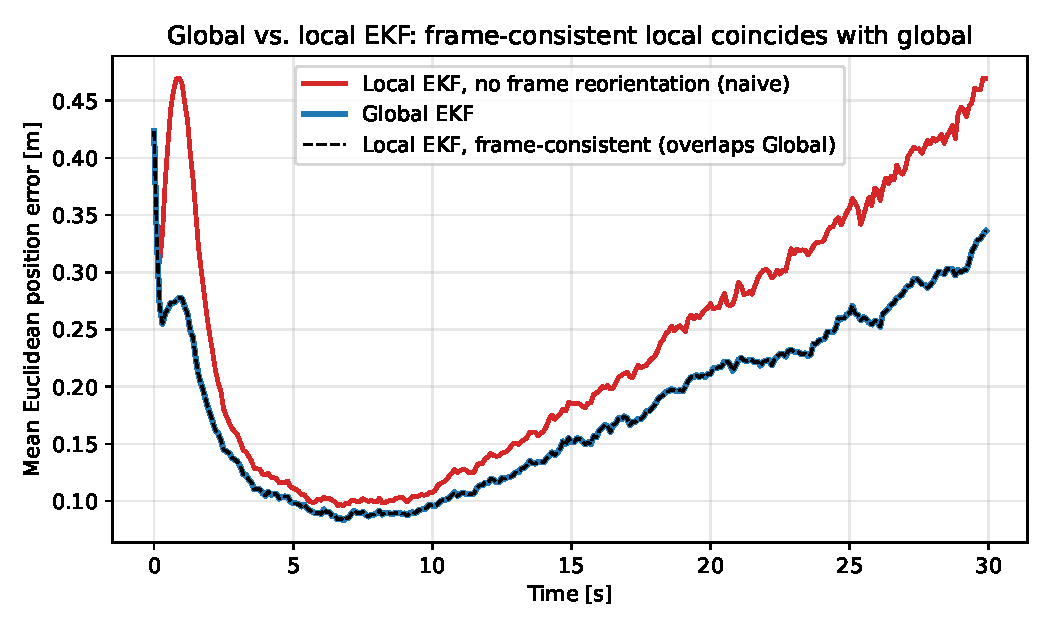
\includegraphics[width=0.82\linewidth]{Cap5/ekf_equivalence.pdf}
  \caption{Mean Euclidean position error over time. The global EKF and the
  frame-consistent local EKF coincide to machine precision (blue and dashed
  black). A local EKF that ignores the inter-frame reorientation
  (Section~\ref{sec:diverge}) is markedly worse (red).}
  \label{fig:ekf_equiv}
\end{figure}

\section{When the Formulations Diverge}
\label{sec:diverge}

Equivalence is a consequence of the three assumptions of
Proposition~\ref{prop:equiv}. Removing any of them yields a genuine difference,
and understanding these regimes is what actually guides the choice of frame.

\subsection{Neglecting Platform Motion}

If the reorientation \eqref{eq:reor_pos}--\eqref{eq:reor_cov} is omitted --- i.e.\
the moving body frame is implicitly treated as inertial --- the prediction is
biased by the platform displacement between consecutive steps. This single
omission raises the RMSE from $0.228$~m to $0.301$~m (the red curve in
Figure~\ref{fig:ekf_equiv}); it does \emph{not} reflect any intrinsic inferiority
of the local frame, but a modelling error. This regime is important precisely
because it can masquerade as a fair ``global versus local'' comparison and
produce a spurious advantage for the global formulation; the correct local filter
recovers the global filter's accuracy exactly.

\subsection{Anisotropic Process Noise}

Assumption~(ii) fails when the acceleration noise is directional in the inertial
frame --- for instance, a target that accelerates predominantly along its track.
Then $\bm{T}_k\bm{Q}\bm{T}_k^{\top}\neq\bm{Q}$, and the formulation whose frame
diagonalises $\bm{Q}$ is preferred: the global filter models inertial-frame
directional noise correctly, whereas the local filter injects it in the rotating
frame and is mismatched. With a strongly anisotropic intensity
($\sigma_{a,x}=0.6$, $\sigma_{a,y}=\sigma_{a,z}=0.05~\mathrm{m/s^2}$) and a
platform yawing at $0.6~\mathrm{rad/s}$, the global filter attains an RMSE of
$0.380$~m against $0.534$~m for the local filter --- a $41\%$ degradation
(Figure~\ref{fig:aniso}). Symmetrically, noise that is diagonal in the body frame
favours the local formulation. The guiding principle is to carry the state in the
frame where the process noise is naturally uncorrelated.

\begin{figure}[H]
  \centering
  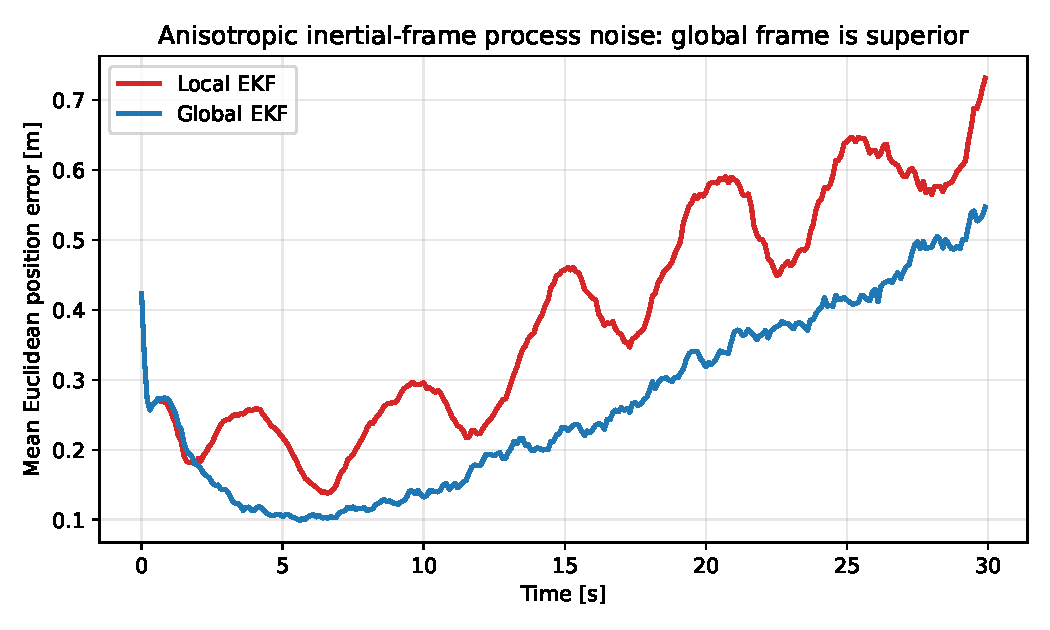
\includegraphics[width=0.82\linewidth]{Cap5/aniso_divergence.pdf}
  \caption{With anisotropic inertial-frame process noise and significant platform
  rotation, the equivalence breaks: the global EKF correctly models the
  directional acceleration noise and outperforms the local EKF.}
  \label{fig:aniso}
\end{figure}

\subsection{Uncertain Platform Pose}

Assumption~(i) is the most consequential in practice. When the platform pose is
\emph{estimated} rather than known, $(\bm{R}_k,\bm{p}^{p}_k)$ carry their own
uncertainty, which enters the global measurement equation \eqref{eq:hglobal} and
the local reorientation \eqref{eq:reor_pos} differently. The innovation covariance
\eqref{eq:gSK} must then be augmented with a term that propagates the pose
covariance, and the two formulations are no longer equivalent. This is the
setting of Chapter~\ref{cha:monocular}, where the monocular tracker explicitly propagates the
six-degree-of-freedom camera-pose uncertainty into the filter.

\section{Cram\'er--Rao Lower Bound}
\label{sec:crlb}

To benchmark the filters against the best achievable accuracy, we compute the
posterior Cram\'er--Rao bound (PCRB) for the discrete-time nonlinear
filtering problem \cite{tichavsky1998}. The Fisher information matrix obeys the
recursion
\begin{equation}
  \bm{J}_{k+1} = \big(\bm{F}\,\bm{J}_k^{-1}\,\bm{F}^{\top} + \bm{Q}\big)^{-1}
              + \mathbb{E}\!\big[\bm{H}_{k+1}^{\top}\,\bm{R}_{k+1}^{-1}\,\bm{H}_{k+1}\big],
  \label{eq:fim}
\end{equation}
where the expectation is taken over the state trajectory --- approximated by
Monte~Carlo, with $\bm{H}_{k+1}$ and $\bm{R}_{k+1}$ evaluated along each true
trajectory --- and the position bound is read off the inverse,
\begin{equation}
  \mathrm{PCRB}(k) = \big[\bm{J}_k^{-1}\big]_{1:3,\,1:3}.
  \label{eq:crlb}
\end{equation}
By Proposition~\ref{prop:equiv} the two formulations share the same bound.
Figure~\ref{fig:crlb} compares, per axis, the empirical RMSE of the filter (over
$3{,}000$ Monte~Carlo runs) with $\sqrt{\mathrm{PCRB}}$. The achieved error
remains at or above the bound at every step --- the filter is near-optimal ---
and the two grow together over time: as the object recedes from the
platform, the range $\rho$ increases and the heteroscedastic term
$\sigma_{\rho}^{2}=\alpha_{\rho}\rho^{2}$ in \eqref{eq:rangenoise} inflates the
measurement uncertainty. This growth is benign for sense-and-avoid: a distant
object poses a lower collision threat, so larger uncertainty at range is
acceptable.

\begin{figure}[H]
  \centering
  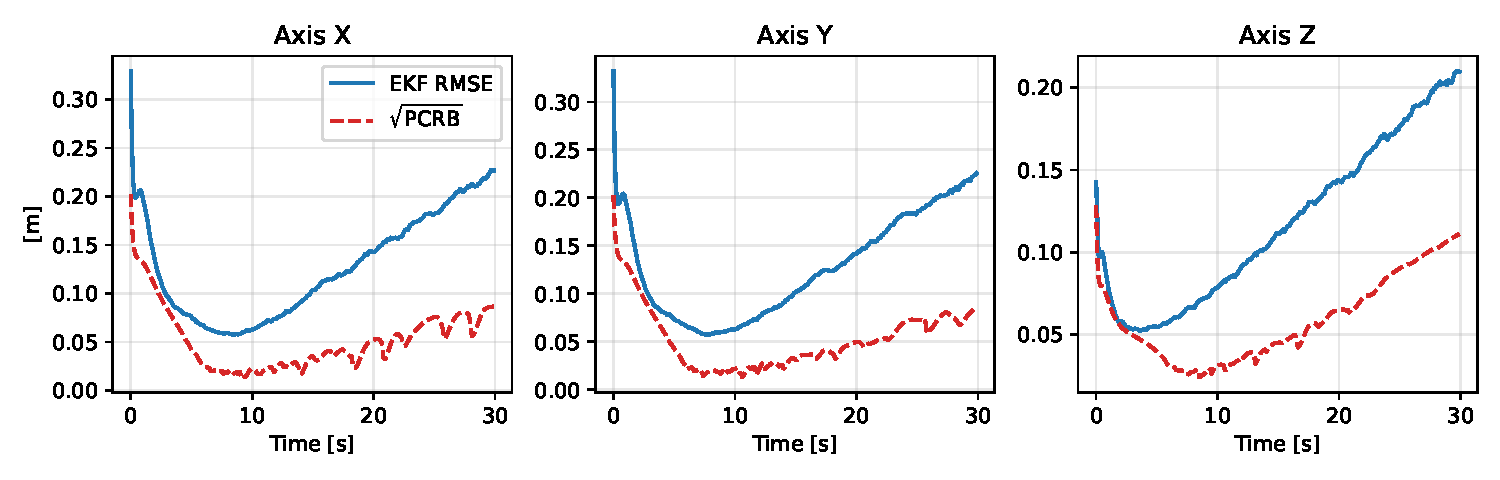
\includegraphics[width=\linewidth]{Cap5/crlb_vs_error.pdf}
  \caption{Per-axis RMSE of the EKF (blue) against the square root of the
  posterior Cram\'er--Rao bound (dashed red), over $3{,}000$ Monte~Carlo runs.
  The achieved error stays at or above the bound at every step; both grow with
  range because of the distance-dependent measurement noise \eqref{eq:rangenoise}.}
  \label{fig:crlb}
\end{figure}
